\section{Storage System Customizing Options in the Cloud}
    \label{sec:options}
    In this section, we discuss several key parameters and related issues in
    setting up customized storage sub-system on cloud-based virtual clusters.

    \subsection{File System Selection}
    \label{subsec:fs}
    A parallel or shared file system is indispensable for parallel program
    execution, which provides a unified persistent storage space to facilitate
    application launching, input and output file accesses, and parallel I/O
    support.  Typically, supercomputers or large clusters are equipped with
    parallel file systems such as Lustre~\cite{lustre},
    GPFS\cite{schmuck:gpfs}, and PVFS~\cite{bib:pvfs}, while smaller clusters
    tend to choose shared/distributed file systems such as NFS.  However,
    end users seldom have the option of choosing or configuring file systems on
    traditional HPC facilities.  One outstanding advantage of cloud HPC
    execution is that users can choose a parallel or shared file system based
    on individual applications' demands, and can switch between different
    selections quite easily and quickly.

    In choosing an appropriate file system, users need to consider their
    applications' I/O intensity and access pattern. For example, a simple NFS
    installation may suffice if the application has little I/O demand, or a
    low I/O concurrency (seen in parallel codes where one process aggregates
    and writes all output data, a rather common behavior in simulations). In
    contrast, applications that write large, shared files usually benefit from
    parallel file systems, especially those heavily optimized for MPI-IO
    operations. Especially, parallel file systems will allow users to scale
    up the aggregate I/O throughput by adding more I/O servers, while the
    single NFS server may easily become a bottleneck under heavy I/O loads.
    Depending on the variability among per-file access patterns, users may
    elect to use file systems that give extra flexibility in performance
    optimization, such as the per-file striping setting allowed by PVFS.

    In our preliminary evaluation presented in Section~\ref{sec:perf}, we
    demonstrate the performance difference of an I/O intensive parallel
    program running on NFS and PVFS, two popular file systems on
    clusters.  Due to the space limit, we confine our discussion here 
    to these two file systems. However, we believe that the
    potential to gain performance and/or cost benefits via storage option
    tuning apply to other file system choices as well.

    \subsection{Storage Device Selection}
    Another important storage parameter is the type of underlying storage
    devices.  Cloud platforms typically provide multiple storage choices, with
    different levels of abstraction and access interfaces. For example, with
    EC2 CCIs, each instance can access three forms of storage: (1) the local
    block storage (``ephemeral'') with 1690GB capacity, where user data are
    not saved once the instances are released, (2) off-instance Elastic Block
    Store (EBS), where volumes can be attached to an EC2 instance as block
    storage devices, whose content persist across computation sessions, and
    (3) Simple Storage Service (S3), Amazon's key-value based object storage,
    accessed through a web services interface.

    For HPC applications, the ephemeral and EBS are more apparent choices as
    storage devices, as they do not require modifications to applications.
    S3, on the other hand, is designed more for Internet or database
    applications and lacks general file system interfaces needed in HPC
    programs.

    Beside data consistency, the ephemeral and EBS devices possess different
    performance characteristics and usage constraints. One instance can only
    mount up to two ephemeral disks, while the number of EBS disks attached
    to it can be almost unlimited.  In our preliminary benchmarking,
    we found the performance gap between the EBS and ephemeral disks 
    small, especially for writes (the major I/O operation in numerical
    parallel programs), as to be demonstrated in Figure~\ref{fig:nfs}.
    However, we observed that the ephemeral disk has better availability and
    lower performance variance. This may be the result of different disk
    affinity and different virtualization techniques. Finally, the ephemeral
    disks are free, while EBS disks are charged by the storage capacity
    consumed.

    Therefore, the choice between these two storage devices again depends on
    the needs of individual applications or users. For instance, production
    runs that generate results to be migrated to and visualized on users' local
    platforms may get the best benefit from using ephemeral disks, as
    persistent storage is not needed. On the other hand, repeated processing
    of the same dataset (such as sequence database searches) will benefit from
    using the EBS. As another example, bandwidth-thirsty applications relying
    on parallel I/O with file striping may suffer from the load imbalance
    introduced by the high performance variability of EBS disks.

    \subsection{File System Internal Parameters}
    \begin{figure}[htpb]
        \centering
        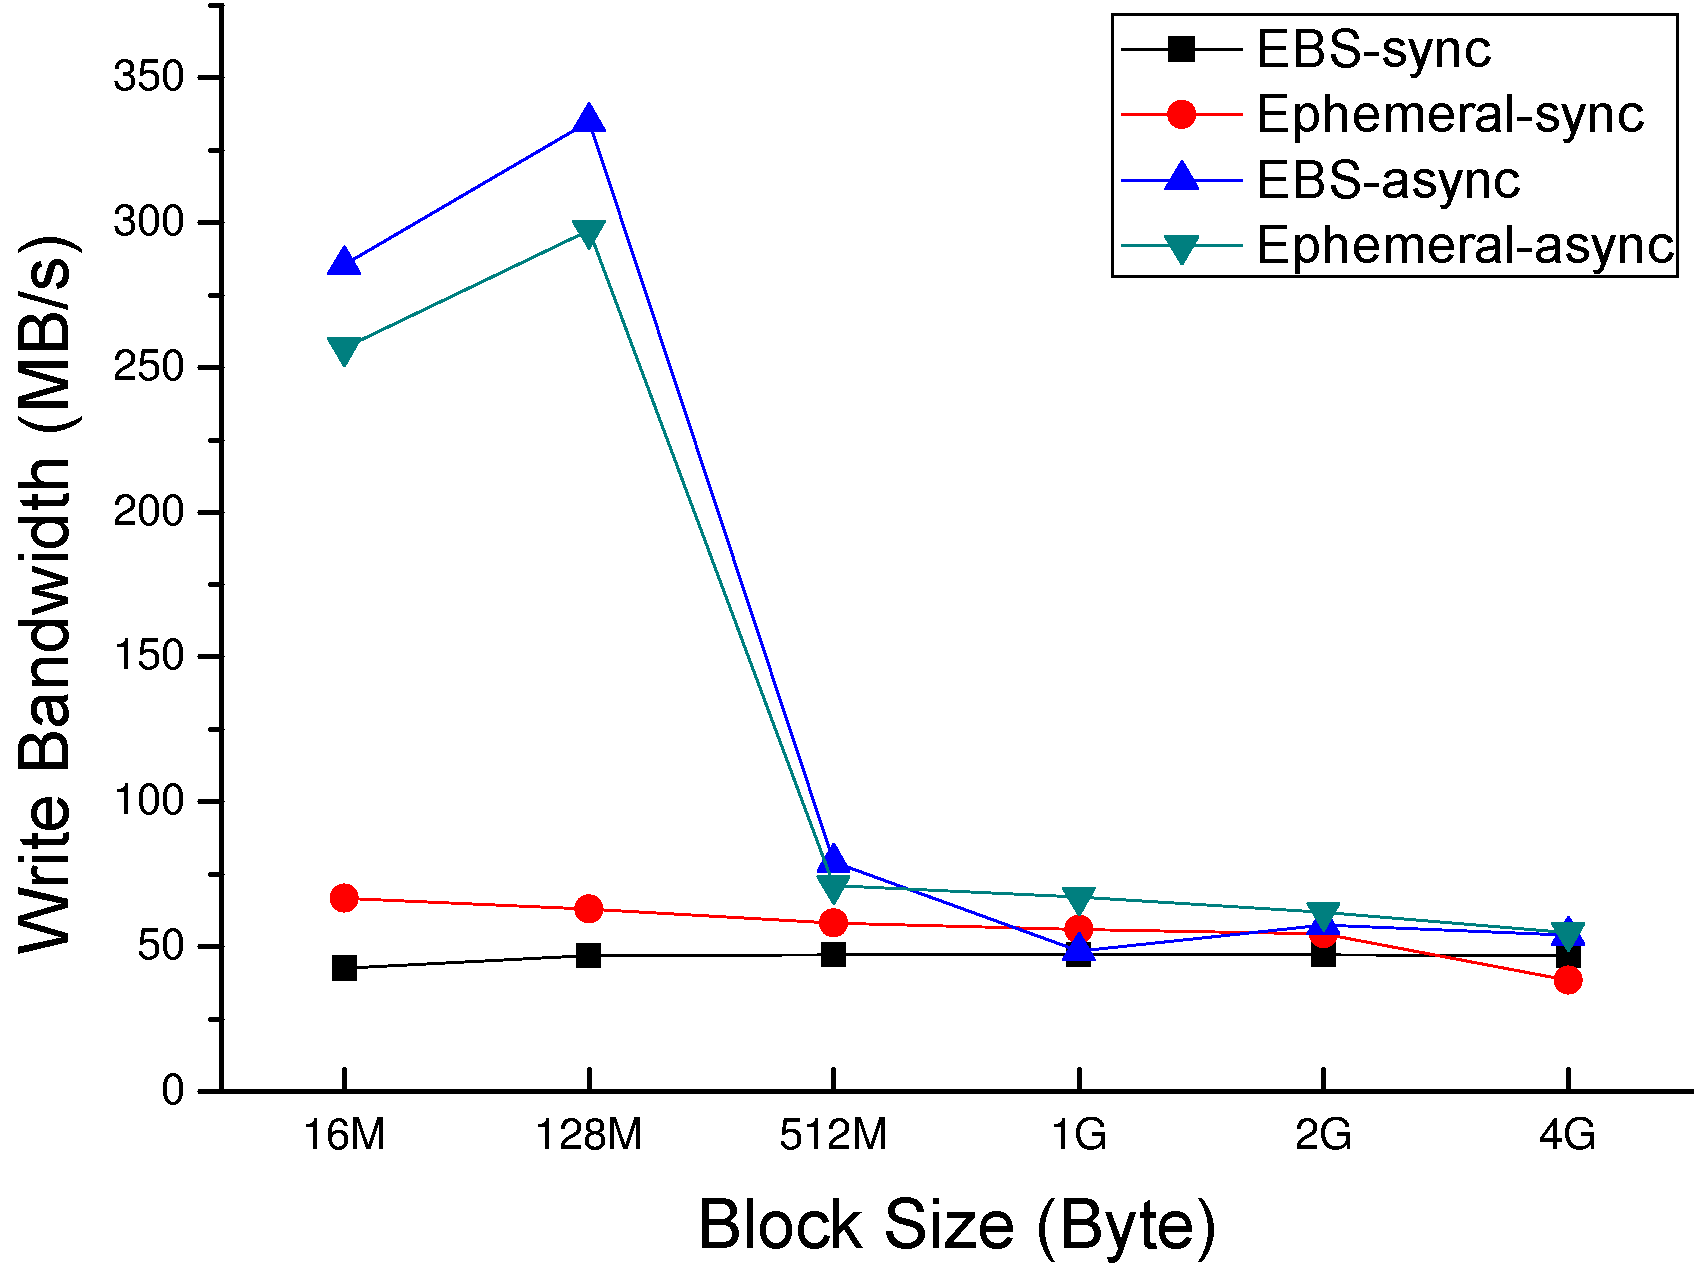
\includegraphics[width=0.8\linewidth]{../figures/nfs-write}
        \caption{NFS write bandwidth, measured with IOR}
        \label{fig:nfs}
    \end{figure}
    For NFS, one sample internal parameter is the choice of write modes:
    \textit{sync} vs. \textit{async}.  Figure~\ref{fig:nfs} shows the results
    from running IOR \cite{bib:ior}, a parallel I/O benchmark, with these
    two modes. We measured the NFS write bandwidth, using two client
    instances, each running 8 IOR processes. The 16 processes write a shared
    file collectively, each dumping a contiguous partition (block).  The block
    size is varied from 16MB to 4GB. As shown in Figure \ref{fig:nfs}, with
    small data blocks, the \textit{async} mode is able to offer a significant
    performance advantage, due to the buffering effect at server side. It will
    be a sound choice for applications that output a moderate amount of data
    and do not require that such data are flushed to secondary storage, such
    as periodic checkpoints (whose loss can be compensated by re-executing a
    certain number of computation timesteps in most numerical simulations). We
    use the \textit{async} mode for NFS server by default in the following
    experiments. 
    \begin{figure}[htpb]
        \centering
        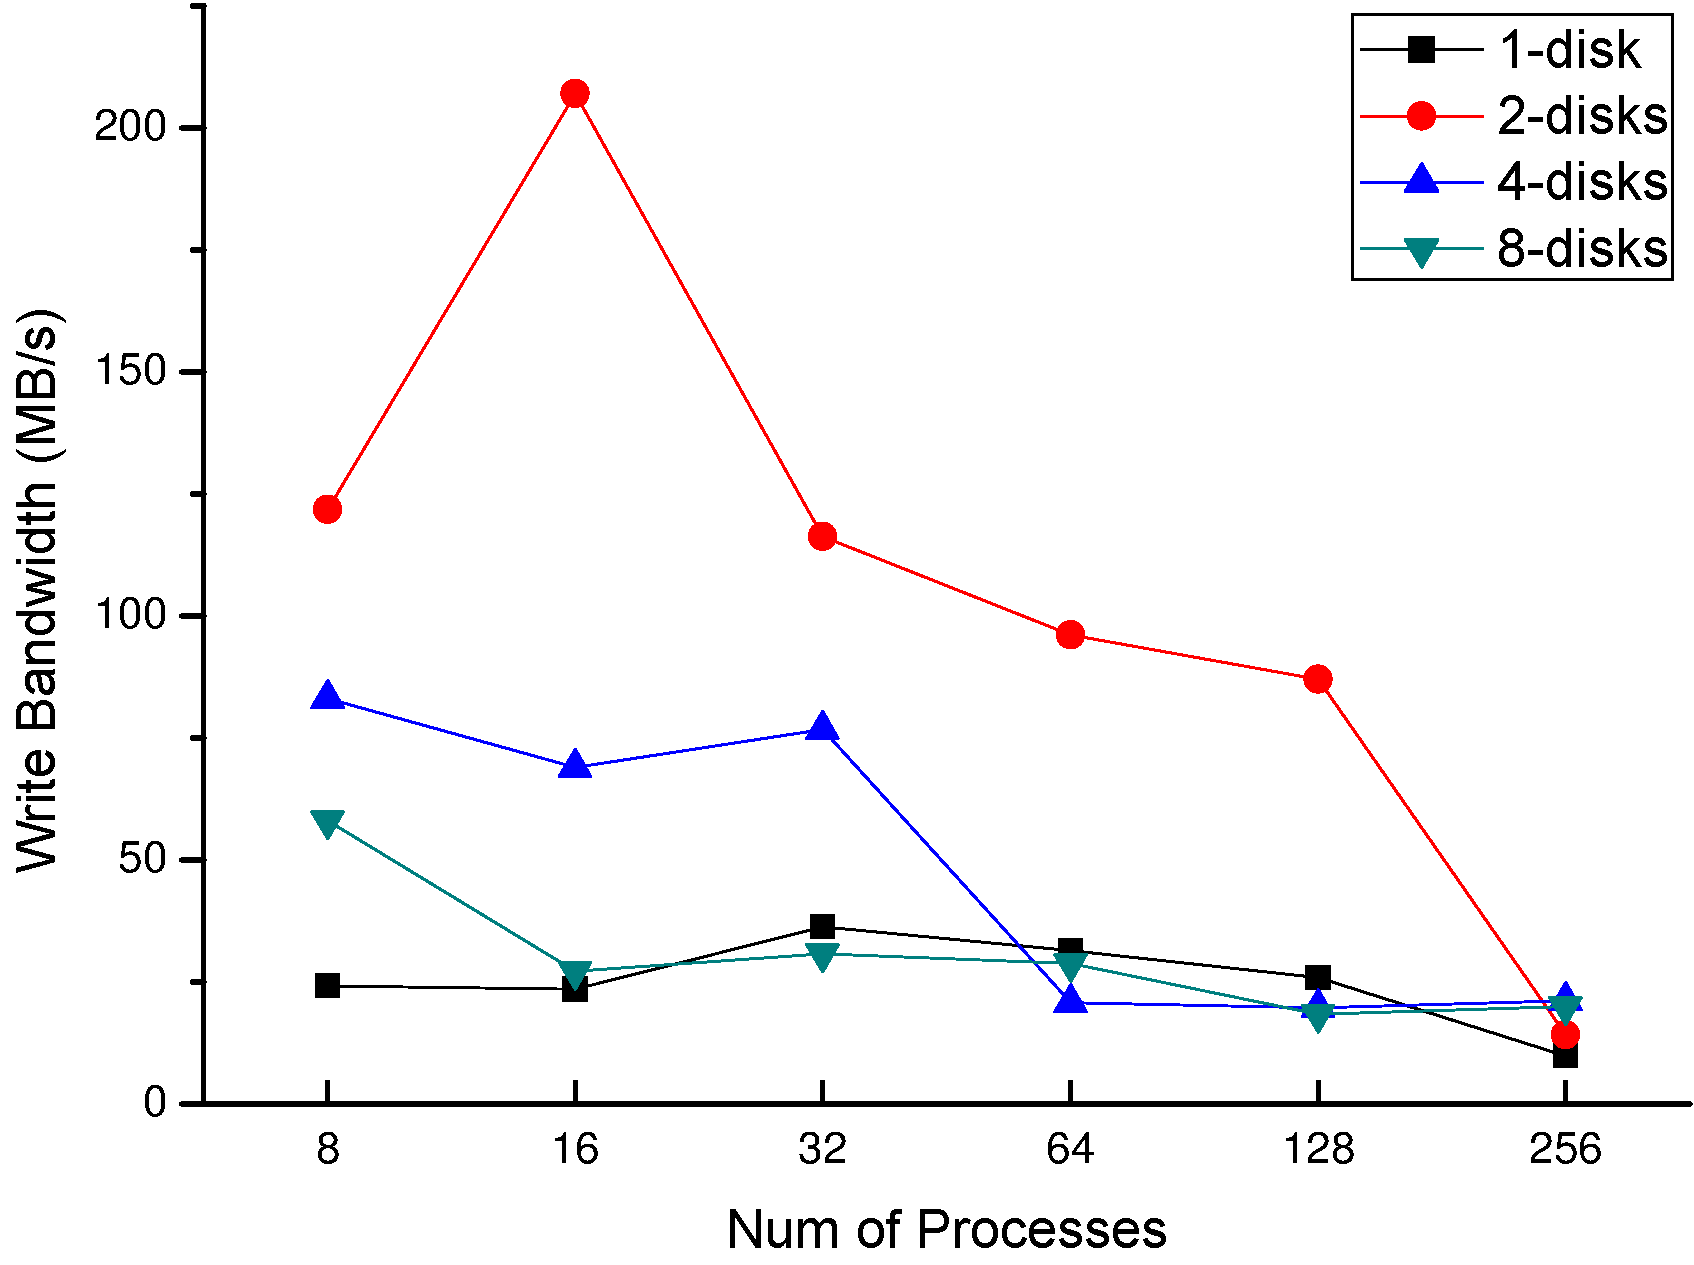
\includegraphics[width=0.8\linewidth]{../figures/nfs-raid0-write}
        \caption{NFS write bandwidth with EBS disks combining into a software RAID0}
        \label{fig:nfs_raid0}
    \end{figure}

    On cloud platforms, a user can have tremendous flexibility in scaling up
    the aggregate I/O capacity and bandwidth, according to the I/O demands of
    their applications. For parallel file systems, this can be done by
    increasing the number of I/O servers, while the NFS could not scale
    because of the single server bottleneck. For all file systems, we can also
    improve each I/O server's capability by increasing the number of disks
    attached to it. One simple way of doing this is to combine multiple disks
    into a software RAID0 partition.  However, one may not obtain expected
    scaling effect when adding (and paying for) more disks to an I/O server.
    Figure~\ref{fig:nfs_raid0} illustrates this with another set of IOR
    collective write experiments, where we fixed the size of data block per
    process (2GB) and varied the number of processes. We evaluated different
    numbers (1, 2, 4, 8) of EBS disks forming a single RAID0 partition on the
    NFS server, and found that the system  hits its peak bandwidth when only
    two disks are mounted. There are many possible reasons for this, such as
    the virtualized layer between storage volumes and multiple users, the
    network connection between the physical node and the physical storage
    devices, and the performance variance of EBS devices. In our future work
    we plan to investigate the disk scaling problem, as a part of automatic
    cloud storage configuration.

    In addition, each file system has many parameters (such as striping factor,
    unit size, metadata server placement and disk synchronization), most of
    which can be configured the same way on both the cloud and the in-house
    cluster platforms.  However, there are exceptions due to the difference in
    usage model brought by the virtualized cluster environment on clouds.  For
    example, the compute resource of an I/O server is not fully utilized if
    the I/O server process occupies an 8-core virtual machine. Unlike on a
    static cluster, where an I/O server is possibly shared among multiple
    applications and/or users, a cloud-based virtual cluster is typically used
    for a dedicated run.  Therefore, it is an interesting problem to explore
    the I/O server and metadata server placement on cloud instances, to
    achieve better resource utilization and overall cost-effectiveness.  In
    Section~\ref{sec:perf} we will report empirical results with sample
    placement settings.
